\chapter{Description Dredging Processes}

INTRO met verwijzingen


\newpage
\section{Sedimentation in hopper \& overflow losses}
\label{sec:hopper}

Research on the sedimentation process is carried out by multiple professors like \citep{Miedema_Vlasblom}, \citep{Ooijens} and \citep{Rhee}. All their models are based on the \citep{Camp} model, a settling basin theory model which was developed for waste water treatment. The Camp model is a strongly simplified flow field where no vertical flow and constant flow depth are assumed. The description of the Camp model is shown in figure \ref{fig:Camp}. It can be seen that all particles having a settling velocity larger than v$_0$ enter the sludge zone and therefore are removed from the flow. Particles having a smaller settling velocity w$_s$ only enter the sludge zone when they enter the settling zone between point b and c.

\begin{figure}[ht!]
    \centering
    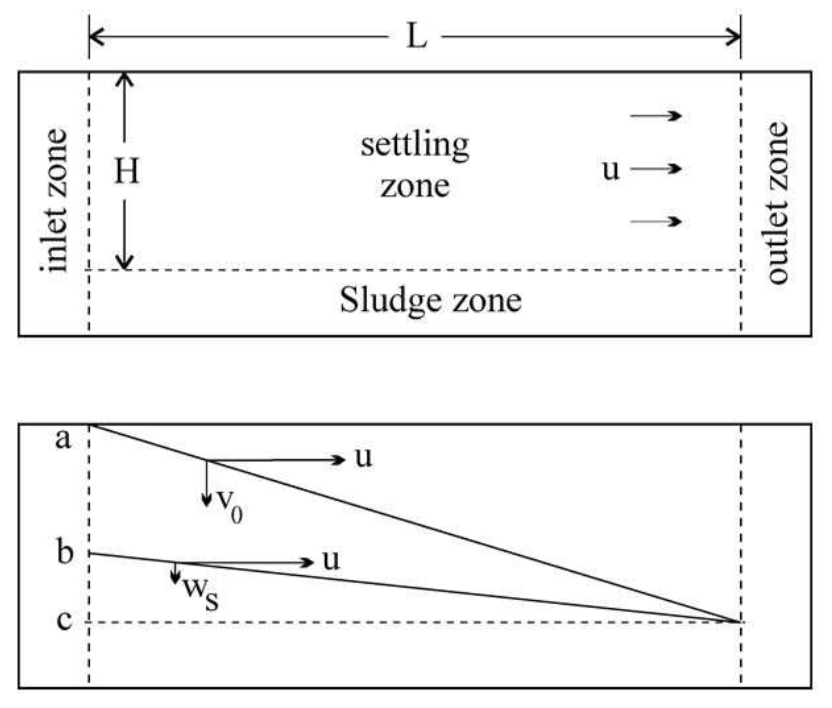
\includegraphics[width=.6\linewidth]{Images/Camp.png}
    \caption{Ideal settling basin according to Camp}
    \label{fig:Camp}
\end{figure}

\noindent \cite{Miedema_Vlasblom} used the Camp model as the basis for their model, but added sorting, erosion, the hindered settling effect and the influence of a rising sand bed. In addition, \cite{Ooijens} added dynamics for example the time effect, which was added by regarding the hopper as an ideal mixing tank. \cite{Miedema_Vlasblom} assumed an equal inflow concentration and concentration in the hopper and a instantaneous reaction of the outflow concentration on the determined settling efficiency. \cite{Ooijens} used the calculated concentration in the hopper for the settling efficiency. \\
\noindent An important quantity during the loading process is the overflow loss. Two different definitions are known. The loss can be defined as the ratio of the total outflow and inflow volume or as the ratio of the outflow and inflow sand flux at a certain moment \citep{Rhee}.\newline \newline
The overflow flux is defined as:

\begin{equation}
\label{eq:OV_flux}
    OV_{flux}(t) = \frac{Q_o(t) C_o(t)}{Q_i(t) C_i(t)}
\end{equation}
\nomenclature[A]{$Q_o$}{Outflow discharge \nomunit{[$m^3/s$]}}
\nomenclature[A]{$Q_i$}{Inflow discharge \nomunit{[$m^3/s$]}}
\nomenclature[A]{$C_o$}{Outflow concentration \nomunit{[-]}}
\nomenclature[A]{$C_i$}{Inflow concentration \nomunit{[-]}}
\nomenclature[A]{$OV_{flux}$}{Overflow flux \nomunit{[-]}}
\nomenclature[A]{$OV_{cum}$}{Cumulative overflow flux \nomunit{[-]}}
\nomenclature[Z]{$OV$}{Overflow Loss}


\noindent The cumulative overflow loss is defined as:

\begin{equation}
\label{eq:OV_cum}
    OV_{cum}(t) = \frac{\int_{0}^{t} Q_o(t) C_o(t) dt}{\int_{0}^{t} Q_i(t) C_i(t) dt}
\end{equation}
\newline
\noindent \textit{Q} is the discharge and \textit{C} the volume concentration. The indices \textit{i} and \textit{o} are related to the inflow and outflow in the hopper \citep{Rhee}. When the sedimentation processes in the hopper are taken into account, the overflow losses can be described as a function of the concentration in the hopper \textit{$C_v$}, the average flow \textit{$Q_{ave}$}, the height of the bed in the hopper \textit{$h_s$}, grain size \textit{$D_{50}$} and the grain size uniformity \textit{$cu$} which is the \textit{$D_{60}$/$D_{10}$} ratio \citep{Ooijens}. Therefore, the overflow loss can be described as:

\begin{equation}
\label{eq:OV}
    OV = f(C_v, Q_{ave}, h_s, D_{50}, cu)
\end{equation} \newline

\noindent However, \cite{Ooijens} assumed a steady state in his model and therefore processes like erosion, local flow and concentration are neglected. \cite{Ooijens} and others distinguished four stages of overflow loss in time as shown in figure \ref{fig:phases_overflow_loss}.

\begin{figure}[ht!]
    \centering
    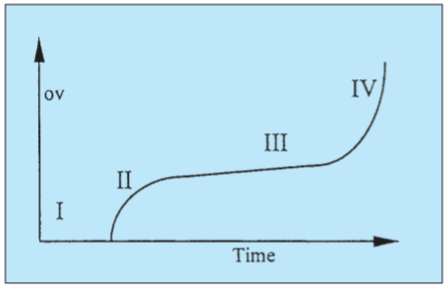
\includegraphics[width=.5\linewidth]{Images/Phases_overflow_loss.png}
    \caption{Stages of overflow losses}
    \label{fig:phases_overflow_loss}
\end{figure}

\begin{enumerate}[I]
    \item Before the overflow level is reached there is no outgoing flow and so, no overflow losses. In this phase the horizontal velocity in the hopper is low, which means good sedimentation of the sediment. The average concentration of the mixture in the hopper will be relatively low when the overflow is reached. The volume during this phase is constant.
    \item Stage II is a transition stage between I and III. When the overflow level is reached, overflowing starts and therefore the velocity in the hopper will increase. The increasing average velocity causes a decreasing settling efficiency. The average concentration in the hopper slowly increases, causing a decreasing settling velocity and an increasing overflow loss. The volume during this phase will decrease.
    \item A steady-state phase emerges in which only the volume of the mixture and the horizontal velocity will slowly increase. The overflow losses are quite constant in this phase, until the scouring velocity is reached.
    \item The horizontal velocity in the hopper will increase and scouring will dominate the settling process when the free volume in the hopper decreases. This increases the overflow losses strongly and decreases the volume in the hopper.
\end{enumerate}

\noindent This theory with different phases is however outdated by the research of \cite{Rhee} where several experiments are carried out in a rectangular laboratory flume with a glass side wall, where flow patterns could be monitored. \cite{Rhee} concluded that the hopper area can be divided into five different sections (figure \ref{fig:overview_hopper_flowfield}), where A is the inflow and B is the density current.


\begin{figure}[ht!]
    \centering
    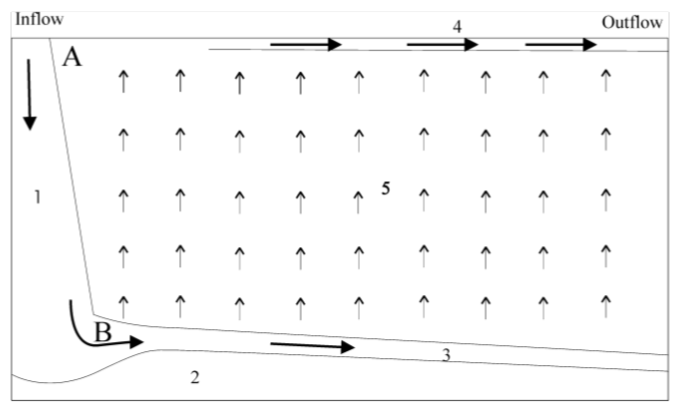
\includegraphics[width=.6\linewidth]{Images/Overview_hopper_flowfield.png}
    \caption{Schematic overview of flow field in hopper.}
    \label{fig:overview_hopper_flowfield}
\end{figure}

\noindent The five different sections are divided in:

\begin{enumerate}
    \item Inflow section
    \item Settled sand / stationary bed
    \item Density flow over settled bed
    \item Horizontal flow at the surface towards overflow
    \item Suspension in remaining area
    
\end{enumerate}

\noindent The incoming mixture (A) flows towards the bottom and forms an erosion crater and density current (B). From this current, sedimentation will take place where coarser particles will settle first which results in a rising bed level. A part of the incoming sediment which does not settle (fine particles) will go up in suspension. When the overflow level is reached, the surface water creates a horizontal current to the overflow. This process is continued until the hopper is completely filled with sediment.\newline \cite{Rhee} measured the the particle size distribution at the inflow and outflow where the overflow samples showed a large variation of particle size distribution, becoming coarser in time. The increasing grain diameter in the overflow is related to the increasing concentration in the overflow. Due to hindered settling, the settling velocity decreases with concentration and therefore larger particles remain in suspension and are removed with the overflow. Also, erosion of the bed at the surface when the hopper is almost totally filled, adds coarser materials to the overflow. \newline
\cite{Rhee} used the observed flow field and grain size distributions to develop a numerical 1DV model to determine the overflow losses. Instead of the Camp model, which uses a horizontal one-dimensional approach with a horizontal supply on one side and overflow on the other. The 1DV model of \cite{Rhee} is a vertical model, where sediment is supplied from the bottom and the overflow is located at the top. In addition, the influence of the hopper load parameter and the mutual interaction of the different grain sizes of the particle size distribution is implemented. The numerical 1DV model was compared with hopper sedimentation tests where a good correlation was shown between the model and the experiments. However, horizontal transport and erosion is not accounted for in the 1DV model and probably scale effects are present. Therefore the model can not be guaranteed to be in agreement with reality. \newline In order to include horizontal transport, \cite{Rhee} extended the 1DV model to a 2DV model. A boundary condition at the interface between the settled sediment and the mixture above had to be formulated for the numerical model. In order to do this, sedimentation tests where done in the laboratory and an empirical relation between the bed shear stress and the reduction of the sedimentation flux was found. This empirical relation was built in the 2DV model, after which the model was validated and found to agree well with laboratory- and prototype measurements.

\nomenclature[Z]{1DV}{One Dimensional}
\nomenclature[Z]{2DV}{Two Dimensional}
%%%%%%%%%%%%%%%%%%%%%%%%%%%%%%%%%%%%%%%%%%%%%%%%%%%%%%%%%%%%%%%%%%%%%%%%%%%%%%%%%%%%%%%%%%%%%%%%%%%%%%%%%%%%%%%%%%%%%%%%%%%%%%%%%%%%%%%%%%%%%%%%%%%%%%%%%%%%%%%%%%%%%%%%%%%%%%

\section{Description of overflow plumes}
\label{sec:plume}
%\textbf{Near-, mid- and far field dredging plume} 

The water-sediment mixture that leaves the overflow may have large ecological impact. This depends on, among other things, how the sediment is distributed when leaving the overflow. Upon release from the bottom of the ship, the water-sediment mixture forms a negative-buoyant plume, which is either mixed directly with the ambient water or behaves as a density current \citep{Winterwerp}. Plumes that are mixed directly are called passive plumes and plumes that behave as a density current are called dynamic plumes. \\\\

\noindent \textbf{Dynamic Plumes} \newline
Dynamic plumes, shown in figure \ref{fig:dynamic_plume} \citep{Dankers}, descend rapidly as a current to the seabed and spread radially across the seabed as a dense plume, slowing down in time and distance as the kinetic energy is lost due to friction. The bulk behaviour of the water-sediment mixture rather than the individual settling velocity is important \citep{Winterwerp}. Because of the rather high (bulk) settling velocity of a dynamic plume, the zone of impact is small.
\begin{figure}[ht!]
    \centering
    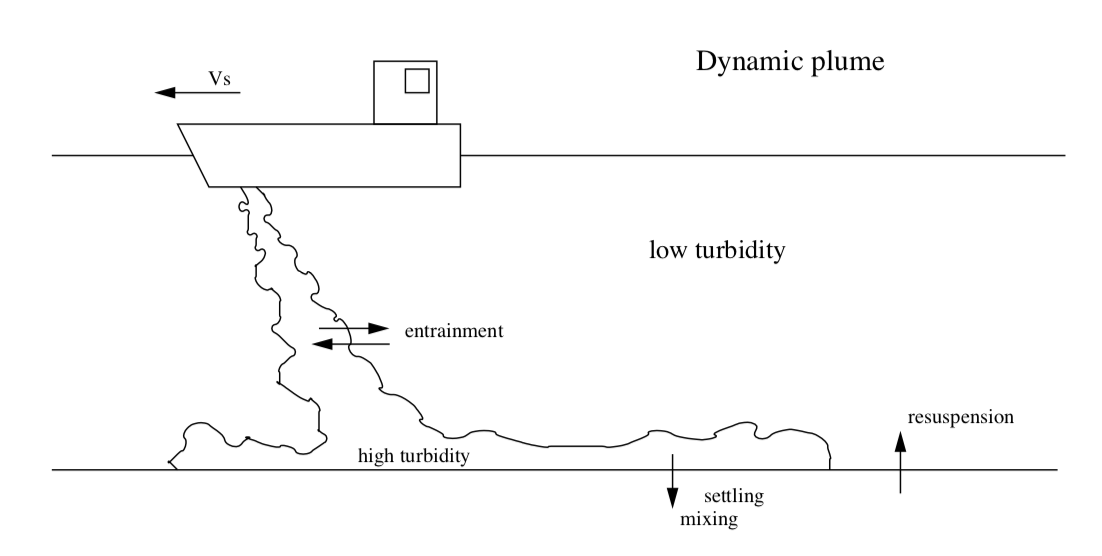
\includegraphics[width=.85\linewidth]{Images/Plume_dynamic.png}
    \caption{Dynamic plume phase }
    \label{fig:dynamic_plume}
\end{figure}

\noindent \textbf{Cloud formation}\newline
A particular case of a dynamic plume develops when the outflow of the overflow is discontinuous. Clouds of sediment, water and air bubbles that entered the overflow due to the discontinuous outflow of the overflow are formed that does not behave as a dynamic plume shown in figure \ref{fig:dynamic_plume}. This phenomena is called cluster settling, convective settling or cloud formation. Clouds can also form from density currents by stretching and eventually 'breaking' in different parts. The cloud formation is presented in figure \ref{fig:cloud_plume} \citep{Dankers}.

\begin{figure}[ht!]
    \centering
    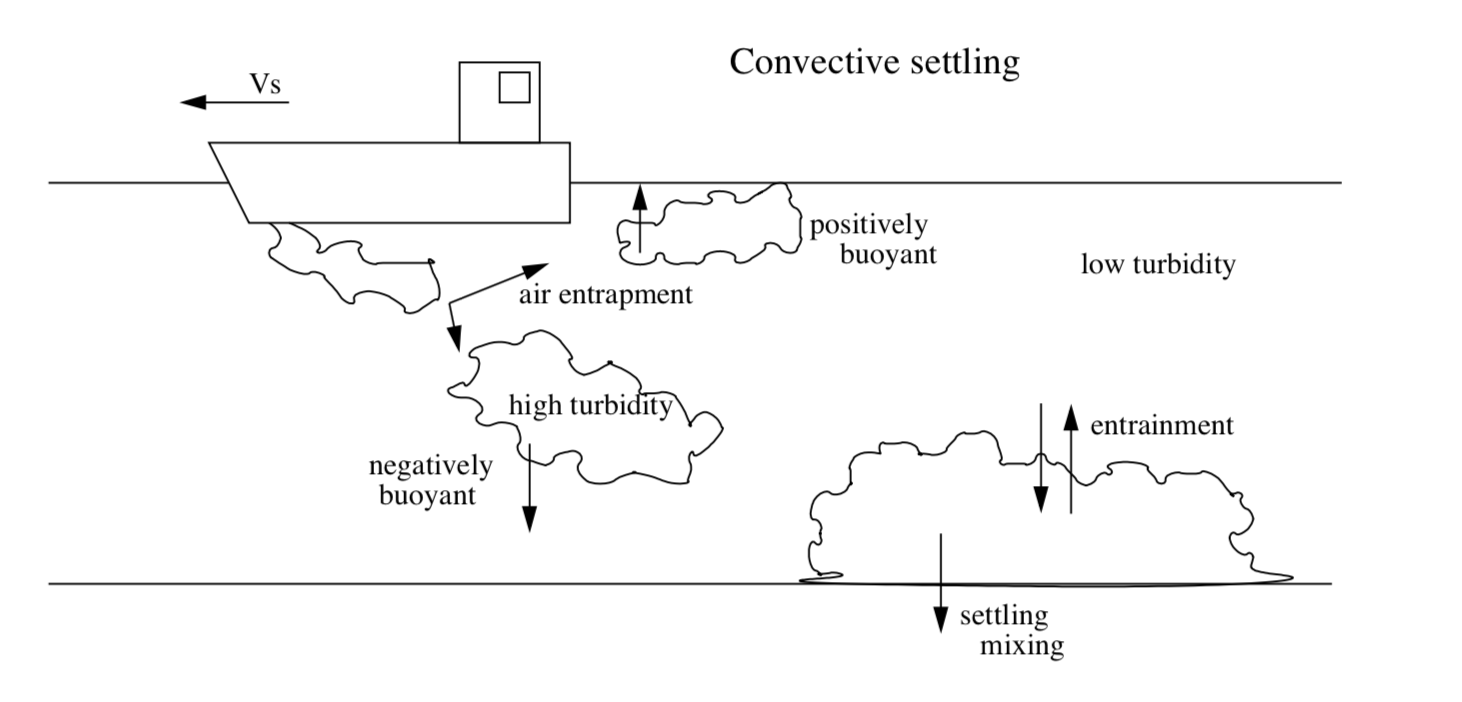
\includegraphics[width=.75\linewidth]{Images/Plume_cloud.png}
    \caption{Plume cloud }
    \label{fig:cloud_plume}
\end{figure}

\newpage
\noindent \textbf{Passive plume} \newline
\noindent
Passive plumes are created due to stripping of dynamic plumes by entrainment caused by turbulence. For example, when the ambient current is strong enough, the plume will be mixed fully with the ambient water. Sediment concentrations are relatively low in a passive plume, therefore fine particles settle extremely slow due to the small settling velocity and the higher depth to the seabed compared to the dynamic plume. The zone of impact of the passive plume is very large and is dependent on the magnitude and direction of the ambient currents. An overview is displayed in figure \ref{fig:passive_plume} \citep{Dankers}.

\begin{figure}[ht!]
    \centering
    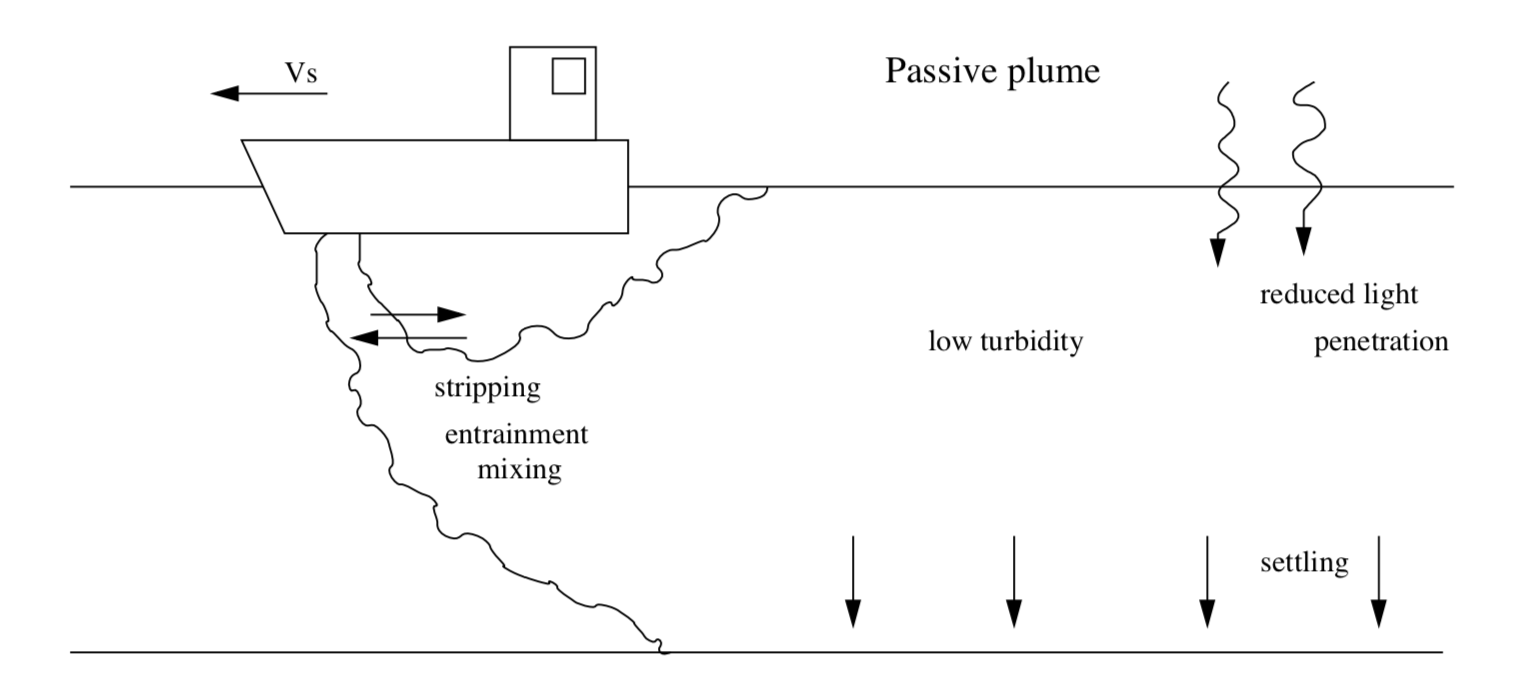
\includegraphics[width=.75\linewidth]{Images/Plume_passive.png}
    \caption{Passive plume phase }
    \label{fig:passive_plume}
\end{figure}




%%%%%%%%%%%%%%%%%%%%%%%%%%%%%%%%%%%%%%%%%%%%%%%%%%%%%%%%%%%%%%%%%%%%%%%%%%%%%%%%%%%%%%%%%%%%%%%%%%%%%%%%%%%%%%%%%%%%%%%%%%%%%%%%%%%%%%%%%%%%%%%%%%%%%%%%%%%%%%%%%%%%%%%%%%%%%%
%Buoyant jet still water Belg 2.3.1
%De wit (2.2) %Belg 2.3.2 
\nomenclature[Z]{JICF}{Jet In Cross Flow}
\label{sec:froudenr}


\section{Turbulent buoyant jet in ambient cross flow}
As mentioned in section \ref{sec:plume}, the outgoing flow of the overflow forms a negative buoyant jet. The ambient current has effect on the buoyant jet, which will be elaborated in this section. In further notice, a dredging plume is noted as an overflow dredging buoyant jet, because it starts with initial buoyancy and momentum where a plume only starts with buoyancy. However, dredging plume fits better in dredging nomenclature.  \newline

\noindent When releasing a momentum- and buoyancy source from a round pipe in ambient fluid with uniform flow velocity and mass density, the round negative buoyant jet in cross flow (JICF) is obtained. As long as the jet starts fully turbulent, mixing of a buoyant JICF is not strongly dependent on the jet Reynolds numbers (Re), but primarily governed by the densimetric Froude number (F$_{\Delta}$) and the jet-to-cross flow velocity ratio ($\lambda$) \citep{Jirka}.

\begin{equation}
\label{eq:Froude}
    F_{\Delta} = \frac{W_0}{\sqrt{D g  \frac{\Delta \rho}{\rho_w}}}
\end{equation}

\begin{equation}
\label{eq:velocity_ratio}
 \lambda = \frac{W_0}{U_{cf}}
\end{equation}
\newline

\nomenclature[A]{$F_\Delta$}{Densimetric Froude number \nomunit{[-]}}
\nomenclature[A]{$W_0$}{Overflow exit velocity \nomunit{$[m/s]$}}
\nomenclature[A]{$U_{cf}$}{Ambient cross flow velocity \nomunit{$[m/s]$}}
\nomenclature[A]{$D$}{Plume source pipe diameter (Overflow outflow diameter) \nomunit{[$m$]}}
\nomenclature[G]{$\Delta \rho$}{Excess mass density of sediment in ambient fluid \nomunit{[$kg/m^3$]}}
\nomenclature[G]{$\rho_w$}{Mass density of water \nomunit{[$kg/m^3$]}}
\nomenclature[G]{$\rho_s$}{Mass density of sediment \nomunit{[$kg/m^3$]}}

\begin{figure}[ht!]
  \centering
    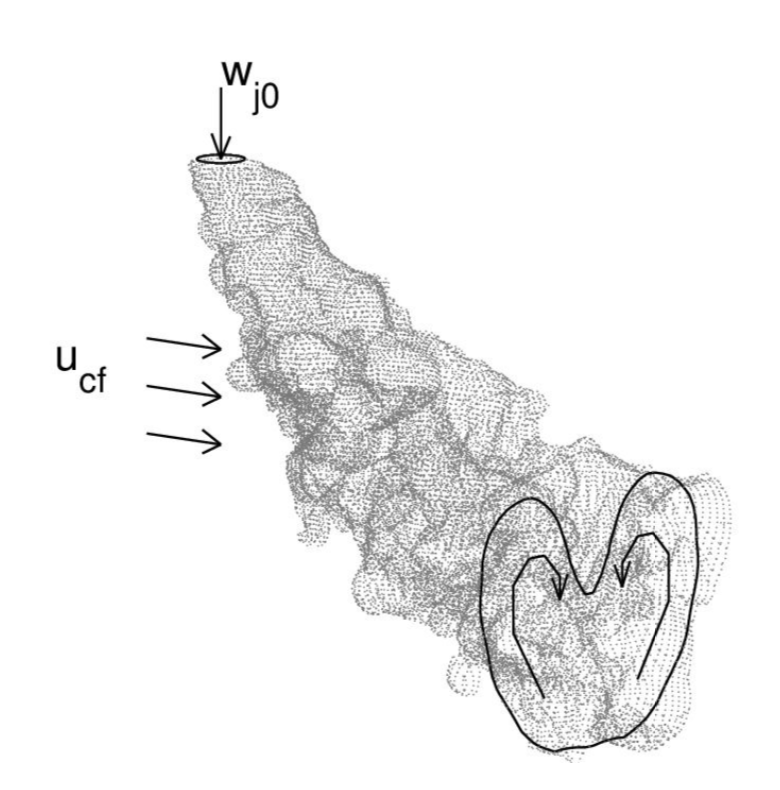
\includegraphics[width=0.4\textwidth]{Images/Jet_mixing.png}
  \caption{Schematic mixing of a negative buoyant JICF }
  \label{fig:Jetmixing}
\end{figure} 

\noindent Where W$_0$ is the overflow exit velocity, U$_{cf}$ is the cross flow velocity (vector sum of dredging speed and ambient current), D the plume source pipe diameter (overflow exit diameter in this case) and $\rho_w$ the mass density of the ambient water. $\Delta \rho$ is the excess mass density of sediment in ambient fluid which also can be described as $\rho_s$ - $\rho$. A schematic overview of mixing of a negative buoyant JICF is shown in figure \ref{fig:Jetmixing} \citep{Dewit}. \newline

\newpage
\noindent The way the plumes spread out is determined by several possible flow regimes \citep{Wright}, \citep{Fischer+}. Jet regime, plume regime and the bent regime are generally found. The jet of a buoyant JICF injected perpendicular to the ambient flow starts with no horizontal velocity. Moving further downstream, the ambient current will take the buoyant plume further in the horizontal. The vertical momentum is important at the exit of the overflow, but eventually buoyancy will take over. \cite{Fischer+} derived length scales to distinguish the different flow regimes of a buoyant JICF. The length scales are given by:

\begin{equation}
\label{eq:lm}
 l_m = \frac{M_0^{3/4}}{B_{0}^{1/2}}
\end{equation}

\begin{equation}
\label{eq:zm}
 z_m = \frac{M_0^{1/2}}{U_{cf}}
\end{equation}

\begin{equation}
\label{eq:zb}
 z_b = \frac{B_0}{U_{cf}^3}
\end{equation}

\begin{equation}
\label{eq:zc}
 z_c = z_m\Big(\frac{z_m}{z_b}\Big)^{1/3} 
\end{equation}

\nomenclature[A]{$B_0$}{Initial overflow buoyancy flux \nomunit{[$m^4/s^3$]}}
\nomenclature[A]{$M_0$}{Initial overflow momentum flux \nomunit{[$m^4/s^2$]}}
\nomenclature[A]{$l_m$}{Jet-to-plume length scale \nomunit{[$m$]}}
\nomenclature[A]{$z_b$}{Buoyancy length scale \nomunit{[$m$]}}
\nomenclature[A]{$z_c$}{Deep water momentum length scale \nomunit{[$m$]}}
\nomenclature[A]{$z_m$}{Momentum length scale \nomunit{[$m$]}}


\noindent $B_0$ is the overflow buoyancy flux and $M_0$ is the overflow momentum flux. As said, the length scales determine the flow regime. If z < $l_m$ from the source, a buoyant jet acts as a jet and when z > $l_m$ the buoyant jet acts as a plume. The length scales $z_m$ \& $z_b$ are defined for the influence of momentum and buoyancy compared to the ambient current. As long as z < $z_m$, initial momentum is dominant over to the ambient current and so the buoyant jet acts like a jet. If z < $z_b$, initial buoyancy is dominant over the ambient current and so acts as plume. \newline
Independent of momentum- or buoyant dominance, a buoyant JICF always ends as a bent over plume due to the horizontal ambient current (figure \ref{fig:Jetmixing}). As long as $z_b$ > $z_m$, the transition to the bent over plume happens after z > $z_b$. In reverse, if $z_m$ > $z_b$, the transition happens after $z_c$. Figure \ref{fig:lengthscales} \citep{Dewit} summaries the length scales and the connected flow regimes of a buoyant JICF, as derived by \cite{Fischer+}.

\begin{figure}[ht!]
    \centering
    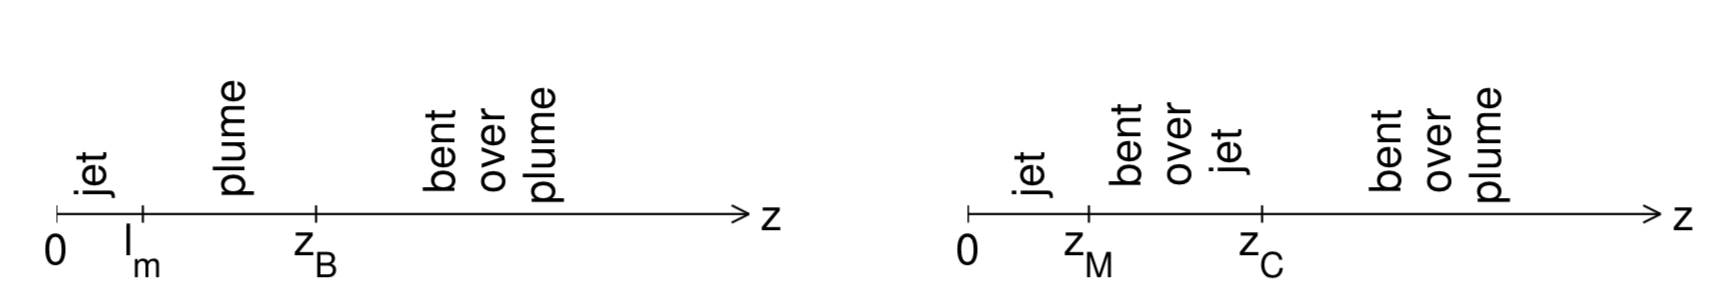
\includegraphics[width=1\linewidth]{Images/Length_scale_z.png}
    \caption{Length scales and flow regimes of a buoyant JICF in case $z_b$ > $z_m$ (left) and in case $z_m$ > $z_b$ (right) }
    \label{fig:lengthscales}
\end{figure}

\noindent The plumes studied in this work correspond to ranges of $F_\Delta$ and $\lambda$ occurring in sediment plumes released from dredging vessels. Even though the initial relative density difference is usually in the order of 1 to 10\%, the buoyancy is relatively weak compared to the cross flow in these cases, with the jet-to-cross flow velocity ratio usually in the range 0.25 < $\lambda$ < 3 \citep{Decrop}. Therefore, the momentum length scale $z_m$ is larger than the buoyancy length scale $z_b$ in most cases, leading to a plume regime sequence as shown in figure \ref{fig:lengthscales} on the right. However, in strong cross flow cases both $z_m$/D and $z_b$/D are around or less than unity, due to which the plume transforms very rapidly to the bent over plume regime.


%%%%%%%%%%%%%%%%%%%%%%%%%%%%%%%%%%%%%%%%%%%%%%%%%%%%%%%%%%%%%%%%%%%%%%%%%%%%%%%%%%%%%%%%%%%%%%%%%%%%%%%%%%%%%%%%%%%%%%%%%%%%%%%%%%%%%%%%%%%%%%%%%%%%%%%%%%%%%%%%%%%%%%%%%%%%%%
%De wit (2.4)

\section{Near field processes dredging plume}

\noindent %\textbf{Near-, mid- and far field dredging plume} \newline
Near field is defined as the zone where plume mixing is dominated by density differences and interaction with the dredging vessel. Typically, the near field zone ends some hundred meters behind the TSHD. In the far field, plume mixing is mainly governed by sediment settling and ambient (tidal) currents \citep{Dewit}. \newline The focus of this study is plume mixing in the near field, because near field mixing determines the amount and distribution of suspended sediment available in the far field. An overview is shown in figure \ref{fig:field}\citep{Dewit}.

\begin{figure}[ht!]
    \centering
    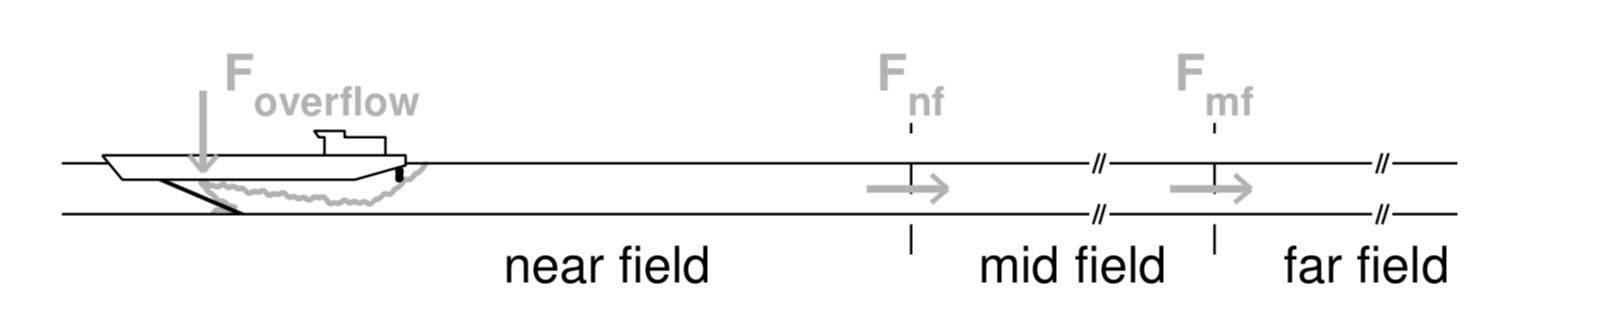
\includegraphics[width=1\linewidth]{Images/Nearfield_Midfield_Farfield.png}
    \caption{Schematic overview of near-, mid- and far field dredging plume. }
    \label{fig:field}
\end{figure}

\noindent The dredge plume normally contains a non-uniform sediment grain size distribution. The sediment particle diameter ($D_p$) can range from sand ($D_p$ > 63 $\mu m$) to mud ($D_p$ < 63 $\mu m$). However, due to the slower settling of finer sediment in the hopper with respect to coarser sediment, the overflow and therefore the exiting plume generally contains more mud and finer particles than the dredged material \citep{Rhee}. \newline
\noindent Under influence of turbulence and differences in settling velocity, mud particles can cluster together to form flocs with typical sizes of 0.01-1mm. The density of mud flocs is less than the density of individual mud particles, however the settling velocity is larger. Flocculation is especially important when the mud concentration is large and therefore strong flocculation has been found for mud fractions inside an overflow plume with floc diameters of 40 - 800$\mu m$ and floc settling velocities of 0.1 - 6mm/s \citep{Smith+}. Even after flocculation, the mud settling velocity is very small leading to large deposition periods, especially for the mud in the surface plume which can take hours to days before it has deposited at the seabed. Although the overflow plume leaves the vessel at the keel several meters below the water surface, the initial velocity is downward and it is denser than the ambient water (it is negatively buoyant). Already close behind the dredger, a part of the overflow plume can end up fully mixed near the water surface as a surface plume where a surface plume can remain visible for considerable distances from a dredger \citep{Newell+}. \newline \newline
\noindent Generally, buoyant JICF mixing is not responsible for the generation of a surface plume, as it will bring the plume further down - not up. Therefore, other processes are responsible for the generation of a surface plume. All theses processes are further elaborated in chapter \ref{CH:influence_factors}.

\nomenclature[A]{$FF_{nf}$}{Near field suspended fine sediment flux (ratio with $FF_{OV}$) \nomunit{[-]}}
\nomenclature[A]{$FF_{mf}$}{Mid field suspended fine sediment flux (ratio with $FF_{OV}$) \nomunit{[-]}}
\nomenclature[A]{$FF_{OV}$}{Suspended fine sediment flux through overflow ($FF_{overflow})$\nomunit{$[kg/s]$}}